\documentclass[12pt]{article}
\usepackage{amssymb,amsmath,graphicx,mathtools}
\usepackage{listings}
\usepackage[margin=0.75in]{geometry}
\parindent 16 pt
\usepackage{fancyhdr}
\usepackage[hidelinks]{hyperref}
\usepackage[usenames,dvipsnames]{xcolor} % Required for custom colors
\usepackage{listings}
\usepackage{float}
\usepackage{sectsty}
\usepackage[bottom]{footmisc}
%\pagestyle{fancy}
%\fancyhead[R]{Imad Ali}
%\fancyhead[L]{Bayesian Win Probability in Basketball}
\DeclarePairedDelimiter\ceil{\lceil}{\rceil}
\DeclarePairedDelimiter\floor{\lfloor}{\rfloor}

\sectionfont{\sffamily\bfseries\upshape\large}
\subsectionfont{\sffamily\bfseries\upshape\normalsize}
\subsubsectionfont{\sffamily\mdseries\upshape\normalsize}

\definecolor{links}{HTML}{FF6688}

\lstset{
    language=R,
    basicstyle=\scriptsize\ttfamily,
    stepnumber=1,
    numbersep=5pt,
    showspaces=false,
    showstringspaces=false,
    showtabs=false,
    frame=single,
    tabsize=2,
    captionpos=b,
    breaklines=true,
    breakatwhitespace=false,
    escapeinside={},
    keywordstyle={},
    morekeywords={}
    }

\title{Bayesian Alternatives to Statistical Significance}
\author{Imad Ali\thanks{National Basketball Association} \and Jonah Gabry\thanks{Columbia University}}

\begin{document}
\maketitle
\abstract{\noindent This paper outlines common misconceptions of Frequentist approaches to statistical significance and proposes a more intuitive Bayesian alternative. At a high-level Frequentist methods focus on the distribution of the test statsitic as opposed to the parameter of interest, whereas the methods proposed here allow the researcher to perform inference directly on the parameter of interest.}
\tableofcontents
\newpage
% CaUSTOM SHORTCUTS

\def\ci{\perp\!\!\!\perp}
\def\ex{\mathbb{E}}
\def\prob{\mathbb{P}}
\def\ind{\mathbb{I}}
\def\grad{\triangledown}
\def\bigo{\mathcal{O}}

\section{Introduction}

Some literature reviewy stuff. Look into Kruschke (might have something on t-tests). Also look into Blitzstein maybe? \\

\noindent In the following section we discuss common misconceptions surrounding test statistics, p-values, and generally speaking the misuse of the term statistical significance. The following section discusses what statistical significance and p-values mean using the one sample t-test as an example. We then show an alternative approach to both the one sample and two sample t-test using the Bayesian framework to evaluate a meaningful difference in parameters.\footnote{We use the term \emph{meaningful} instead of \emph{significant} to avoid confusion since the latter term as been adopted by Frequentists to indicate a meaninful difference in parameters.} Finally, we extend this further to show how we can deal with the significance of parameters in generalized linear regression models. \\

\subsection{Misinterpreting statistical significance}

\noindent A quantity is defined to be statistically significant if the test statistic computed with this quantity is unlikely to occur under the null hypothesis, where the null hypothesis assumes that there is no material difference between the quantity and its hypothesized value. What this means is that if we repeatedly draw samples from the population under the null hypothesis, compute the same statistic, and plot the empirical distribution of the statistic; then the statistic we computed from our original data would fall somewhere in the tails (i.e. a low probability region). One way to quantify this is to compute the proportion of the distribution that is in the tails from the computed test statistic. This quantity is known as a p-value and tells you the probability of computing a statistic under the null hypothesis that is as extreme as the one at hand. Lower p-values indicate that the computed test statistic is way out in the tail(s) of the distribution. \\

\noindent In this discussion of statistical significance we have been talking about quantities that we, as applied researchers, are not really interested in; test statistics and p-values. We are more interested in the underlying quantities used to compute these statistics (in the case of a one sample t-test this is the mean of the data). \\

\section{Inference on Sample Parameters}

It is easier to talk about the process of inference in context so the one sample t-test is used as an example. First we will show how statistical significance is determined using the test and then we will outline a Bayesian alternative by modeling the data using \textbf{rstan}, the R interface to the Stan probabilistic programming language. \\

\noindent Below we have a sample of ten $x$ observations generated from $\mathcal{N}(\mu = 4.5, \sigma = 2)$. The parameter $\mu$ is the population mean and the parameter $\sigma$ is the population standard deviation.

\begin{verbatim}
  x <- c(5.820883, 2.667825, 3.332511, 3.388233, 7.976444,
         5.925112, 6.465919, 7.064625, 3.012066, 2.771472)
\end{verbatim}

\subsection{One Sample t-test}

The \emph{one sample t-test} is used to test the whether the mean of a sample of data $\mu_s$ is significantly different from some hypothesized value $\mu_0$. To avoid confusion, note that $\mu_0$ differs from $\mu$ in that $\mu$ is typically unknown whereas $\mu_0$ is chosen by the researcher depending on the context of the problem. The test statistic associated with this test assumes that data $x$ is generated from the normal distribution and is calculated as,

$$
\mbox{t-statistic} = \frac{\mu_s-\mu_0}{\sigma_s/\sqrt{n}}
$$

\noindent where $\sigma_s$ is the standard deviation of the data $x$ and $n$ is the sample size of the data. This statistic follows the t-distribution with $n-1$ degrees of freedom. \\

\noindent Suppose we want to test whether the mean of these data is statistically different from a hypothesized value $\mu_0 = 4.5$. This is a two-tailed test since we are interested in determining whether the mean is significantly greater than 4.5 or significantly less than 4.5. Applying the t-statistic formula to the data yields the following value,

$$
\frac{4.84-4.5}{2.01/\sqrt{10}} \approx 0.5394
$$

\noindent Since we are dealing with a two-tailed test our test statistics of interest are $\mid 0.5394 \mid$ and $-\mid 0.5394 \mid$. As mentioned in the introduction, we want to determine how unlikely it is to compute test statistics more extereme than the one we have computed. This is done by using the cumulative distribution function for the t-distribution $F(q, \nu)$ parameterized by quantity $q$ and degrees of freedom $\nu$. Since the t-distribution is symmetric we can compute the probability of calculating a statistic less than or equal to -0.5394 under the null hypotheis and multiply this value by 2. Performing this computation yields,

$$
2 \cdot F(0.5394, 10-1) \approx 0.6027
$$

\noindent So there is about a 0.6 probability that a test statistic could occur that is more extereme than the one we computed. In other words, if we repeatedly randomly sample 10 observations under the null hypotheis $x \sim \mathcal{N}(4.5, 2)$ and compute the t-statistic with this data, then 60\% of the time we will observe values more extreme than what we calculated with the orginal data sample. That is a high probability and suggests that there may be no material difference between the test statistic computed from the data sample and the test statistics computed under the null hypothesis. Under the Frequentist interpretation, this implies that the mean of our sample is not statistically different from the hypothesized value, 4.5. \\

\noindent The distribution of t-statistics under the null hypothesis can be illustrated by sampling 10 observations from $\mathcal{N}(4.5,2)$ $B$ times, and plotting a histogram of these $B$ t-statistics. The figure below illustrates such a histogram where $B = 10000$.

\begin{figure}[H]\caption[]{Empirical Distribution of t-Statistic}
\centering
\begin{minipage}{0.6\linewidth}
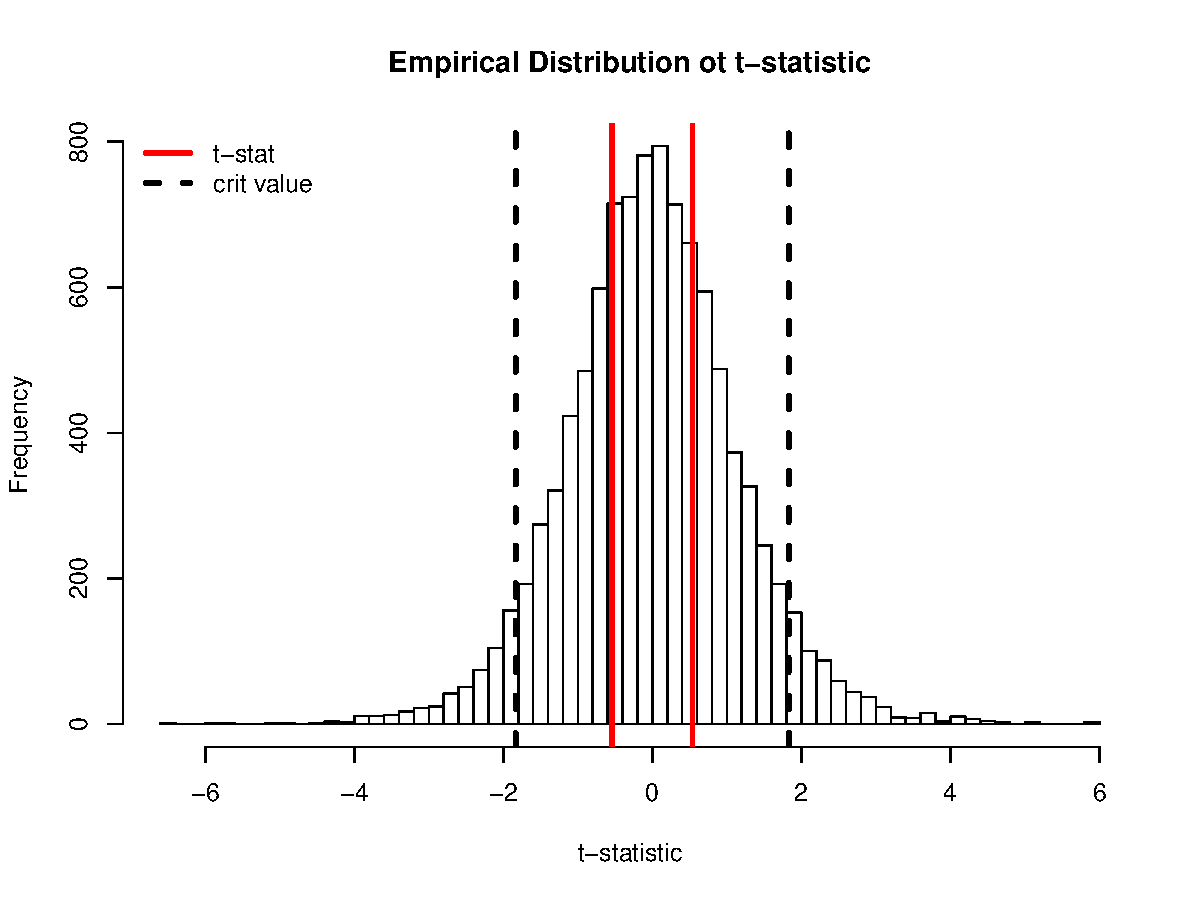
\includegraphics[trim={0cm 0cm 0cm 1.5cm}, clip, scale=0.6]{../figs/ttest_dist.pdf}
\end{minipage}
\end{figure}

\noindent The red lines indicate the t-statistic computed with the data sample provided above. The dashed black lines indicate the critical values where the proportion of the distribution in the tails from those dashed lines is cumulatively 0.1.\footnote{This is an arbitrary choice. The researcher should choose the threshold that is appropriate given the context of the problem.} If our computed t-statistic is outside the critical values then we could say that there is less than 0.1 probability that we would calculate a statistic as extreme as the one we have calculated, suggesting that the statistic is somewhat unique. This tangentially indicates that there is a significant difference between the mean from our data $\mu_s$ and the null hypothesis $\mu_0$. However the statistic falls inside the critical value interval, which leads to the conclusion that $\mu_s$ is not statistically different from 4.5. \\

\subsection{Bayesian alternative to the one sample t-test}

The approach above focused on the test statistic which is derived from the parameter of interest $\mu_s$. The Bayesian alternative to this test involves modeling the data with prior information, and performing inference directly on the parameter estimate $\mu_s$. \\

\noindent In the context of the t-test assumptions the data is modeled using the normal distribution. The prior distributions on the location and scale parameters are up to the researcher. Here, we define normal distributions on both parameters, which gives us the following model,

\begin{align*}
x &\sim \mathcal{N}(\hat{\mu}, \hat{\sigma}) \\
\hat{\mu} &\sim \mathcal{N}(0,3) \\
\hat{\sigma} &\sim \mathcal{N}^{+}(0,3)
\end{align*}

\noindent Fitting this model to the data sample yields samples that define the posterior distribution for $\hat{\mu}$ and $\hat{\sigma}$, along with the posterior predictive distribution $\hat{x}$. Note that the mean of $\hat{\mu}$ is a point estimate and can be thought of as the Bayesian equivalent to $\mu_s$ (similarly for $\hat{\sigma}$ and $\sigma_s$).

\noindent This model equivalent to a regression model where $x$ is the outcome and the only predictor is a single intercept. Redefining the model as a regression problem allows us to estimate the parameters in rstanarm (code below). \\

\begin{verbatim}
            x1 <- c(5.820883, 2.667825, 3.332511, 3.388233, 7.976444,
                    5.925112, 6.465919, 7.064625, 3.012066, 2.771472)
            fit <- stan_glm(x ~ 1, data = x1,
                            prior_intercept = normal(0, 3, autoscale = FALSE),
                            prior_aux = normal(0, 3, autoscale = FALSE))
\end{verbatim}

 The marginal posterior distributions for each of these parameters and the predictions are illustrated in the figure below. The red line illustrates the mean of each of the samples. \\

\begin{figure}[H]\caption[]{Parameter samples given observed data and priors}
\begin{minipage}{1\linewidth}
  \centering
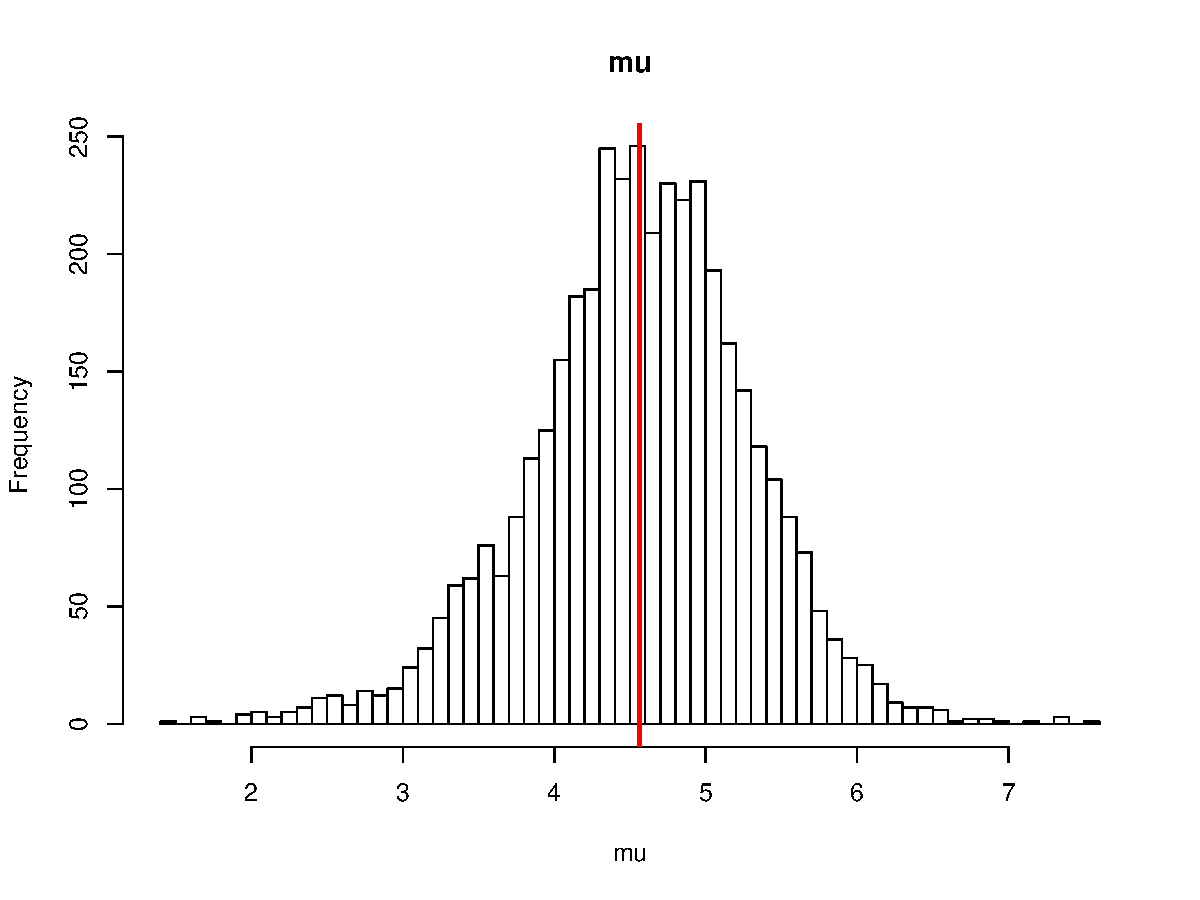
\includegraphics[trim={0cm 0cm 0cm 0cm}, clip, scale=0.4]{../figs/norm1_mu.pdf}
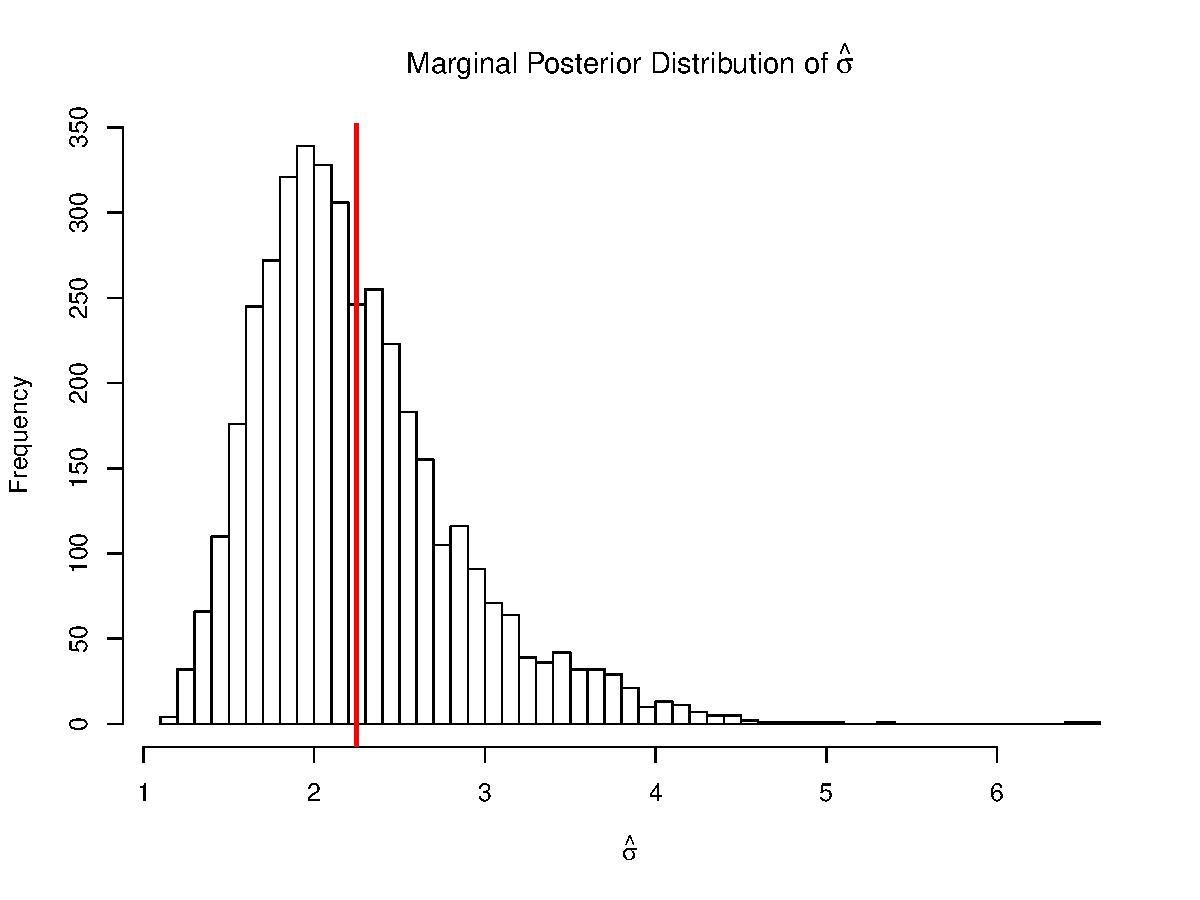
\includegraphics[trim={0cm 0cm 0cm 0cm}, clip, scale=0.4]{../figs/norm1_sigma.pdf}
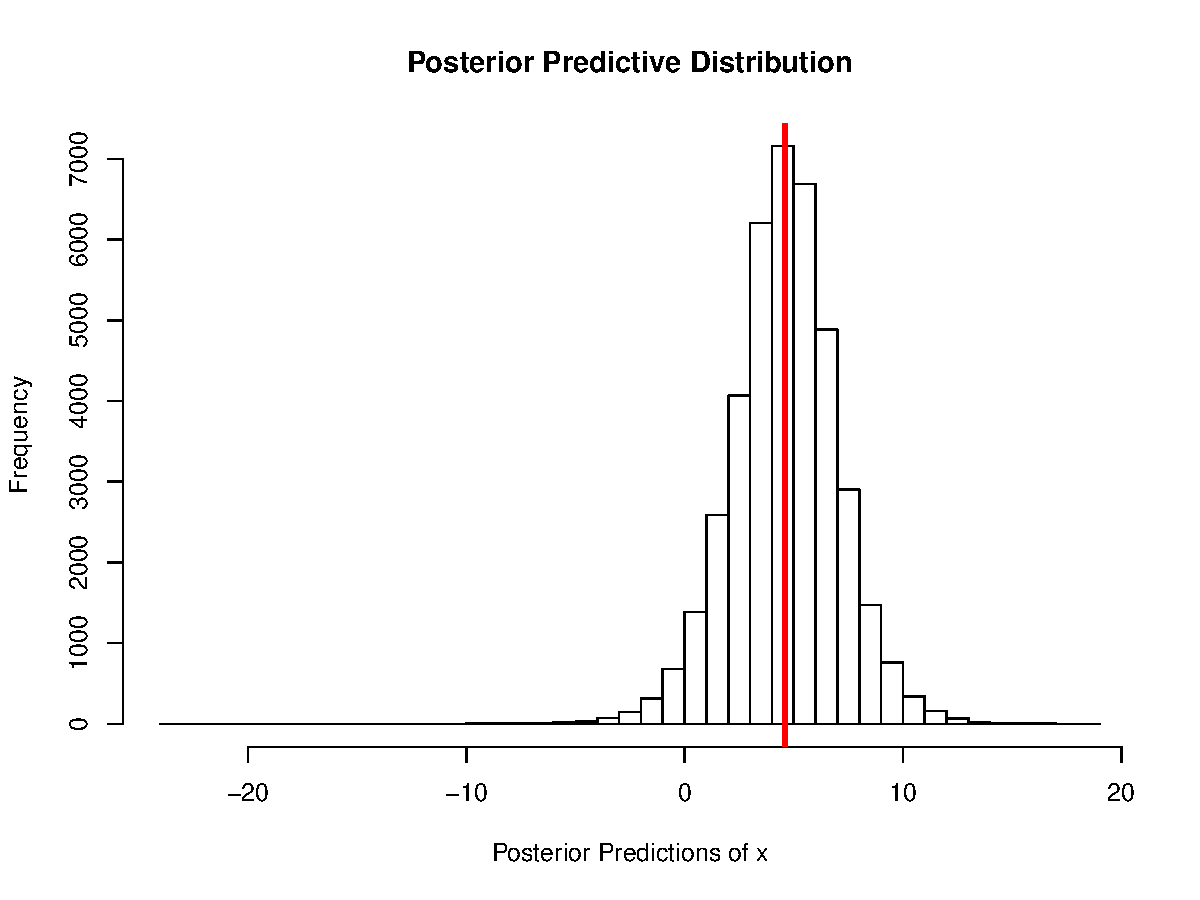
\includegraphics[trim={0cm 0cm 0cm 0cm}, clip, scale=0.4]{../figs/norm1_pp.pdf}
\footnotesize
\end{minipage}
\end{figure}

\noindent We are still interested in testing if the mean is different from the hypothesized value $\mu_0 = 4.5$. To do this we can compute sample quantiles using probabilities defined by the researcher. These \emph{uncertainty intervals} enable us to communicate the probability that the estimated mean is between two values conditional on the data and prior information.\footnote{Uncertainty intervals are also known as credible intervals.} Looking at the figure below, which illustrates the 50\% and 90\% uncertainty intervals for the location parameter, we identify that 90\% of the marginal posterior is between 3.3 and 5.7. It is at the discretion of the researcher to determine whether this interval is satisfactory to probabilistically conclude that the marginal posterior distribution of $\hat{\mu}$ is not different from 4.5. If the 90\% uncertainty interval excluded 4.5 then we could say that there is a 90\% chance that the mean estimated from the sample is different from 4.5. \\

\noindent An analogous approach would be to first take the difference between the samples $\hat{\mu}$ and the hypothesized value $\mu_0$. Then we can compute the quantiles in a similar fashion but would now be interested to know whether or not the 90\% interval contained zero. If it does not then we can be 90\% sure that $\hat{\mu}$ is meaninfully different from $\mu_0$. If the interval does contain zero then the difference between $\mu_0$ and one of the samples was zero indicating that we cannot be 90\% sure that $\hat{\mu}$ is different from $\mu_0$.

\begin{figure}[H]\caption[]{Marginal posterior distribution of $\mu$}
\centering
\begin{minipage}{0.6\linewidth}
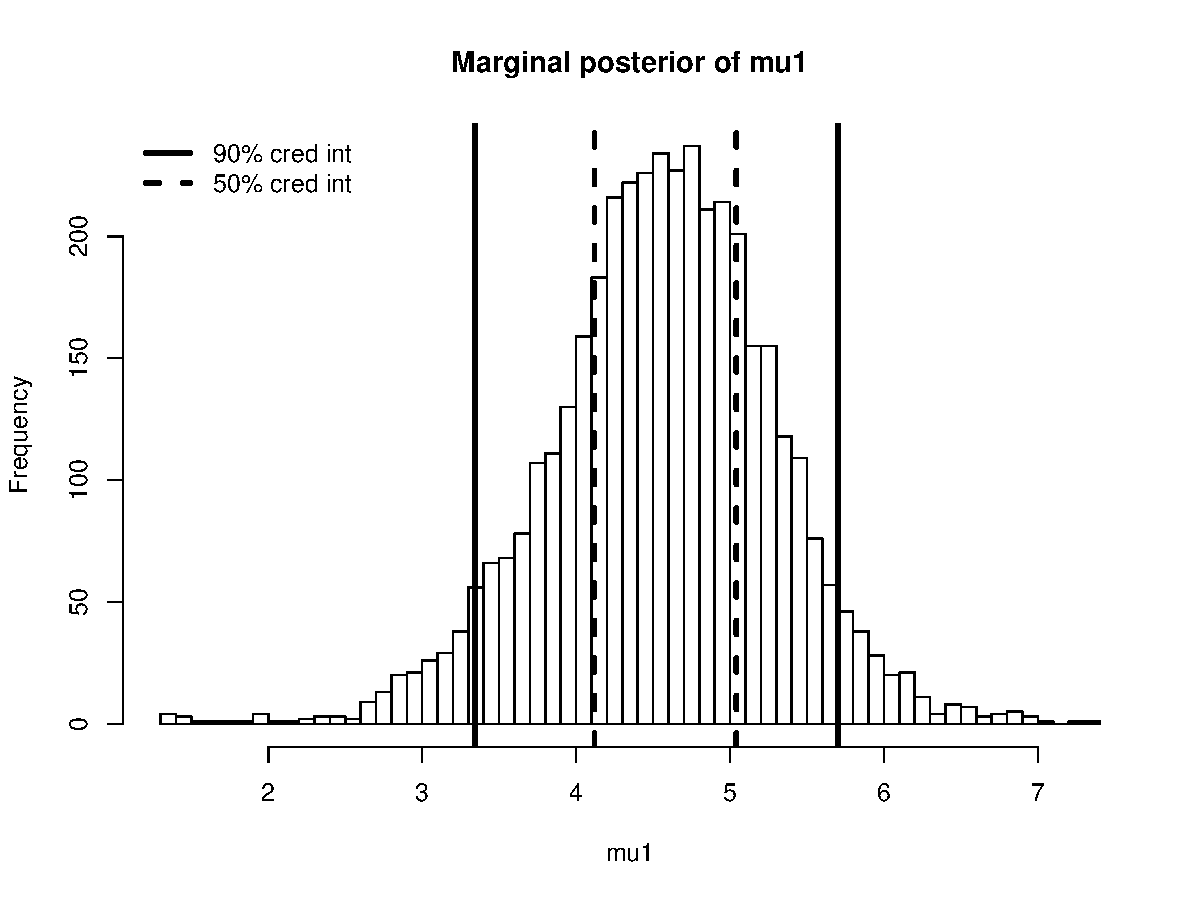
\includegraphics[trim={0cm 0cm 0cm 1.5cm}, clip, scale=0.6]{../figs/norm1.pdf}
\end{minipage}
\end{figure}

\section{Posterior Predictive Distribution}

\section{Conclusion}

\noindent [Conclusion here] \\

\noindent ... \\

\noindent Aside from performing inference directly on parameters, an additional benefit with the Bayesian approach is that it enables researchers to quantify their prior information about the parameters in the model. This is particularly useful for small samples, where prior information has more influence over the marginal posterior distribution of the location parameter. With larger samples more informative priors will need to be defined in order for them to have any substantial influence on the posterior distribution.

\pagebreak

\section{References}

\noindent [References here]

\pagebreak

\section{Appendix - Stan Code}

\noindent The one sample t-test model that was fit using rstanarm can also be fit in rstan by defining the following model in a Stan file:

\begin{verbatim}
               data {
                 int<lower=0> N;
                 vector[N] y;
                 real mu_loc;
                 real sigma_loc;
                 real<lower=0> mu_scale;
                 real<lower=0> sigma_scale;
               }
               parameters {
                 real mu;
                 real<lower=0> sigma;
               }
               model {
                 target+= normal_lpdf(y | mu, sigma);
                 target+= normal_lpdf(mu | mu_loc, mu_scale);
                 target+= normal_lpdf(sigma | sigma_loc, sigma_scale);
               }
               generated quantities {
                 real y_hat[N];
                 for (n in 1:N)
                   y_hat[n] = normal_rng(mu, sigma);
               }

\end{verbatim}

\pagebreak

\section{Appendix - Bayesian Alternative to Two Sample t-Test}

The one-sample approach can be extended to two samples. Suppose we have three data sets ($x_1$, $x_2$, and $x_3$) generated from the normal distribution.

\begin{verbatim}
  x1 <- c(5.820883, 2.667825, 3.332511, 3.388233, 7.976444,
          5.925112, 6.465919, 7.064625, 3.012066, 2.771472)
  x2 <- c(6.329095, 4.575028, 1.346890, 6.440587, 7.479409,
          1.736296, 5.091112, 3.865324, 7.728403, 1.792258)
  x3 <- c(-2.541337, -2.778205, -1.363428, -4.821875, -2.526202,
          -3.587017, -1.073344, -2.400323,  3.287509,  3.278655)
\end{verbatim}

\noindent We want to determine whether the mean of $x_1$ is different from that of $x_2$ and $x_3$. Modeling each set of data according to the approach in the previous section gives the marginal posterior distributions for the location parameters ($\mu_1$, $\mu_2$, and $\mu_3$). We can then compute the 50\% and 90\% quantiles for $\mu_1 - \mu_2$ and $\mu_1 - \mu_3$. For $\mu_1 - \mu_2$ we find that 90\% of the difference in location parameters is between -1.5 and 2.0. This interval contains zero, which means 90\% of the time we cannot confidently conclude that the means of the two samples, $x_1$ and $x_2$ are different. On the other hand the 90\% uncertainty interval for $\mu_1 - \mu_3$ is 4.0 and 7.8 so we can say that 90\% of the time there is a difference between the means of $x_1$ and $x_3$. The figure below illustrates the uncertainty interval for each of these cases.

\begin{figure}[H]\caption[]{Two-sample Inference on Location Parameters}
\begin{minipage}{1\linewidth}
  \centering
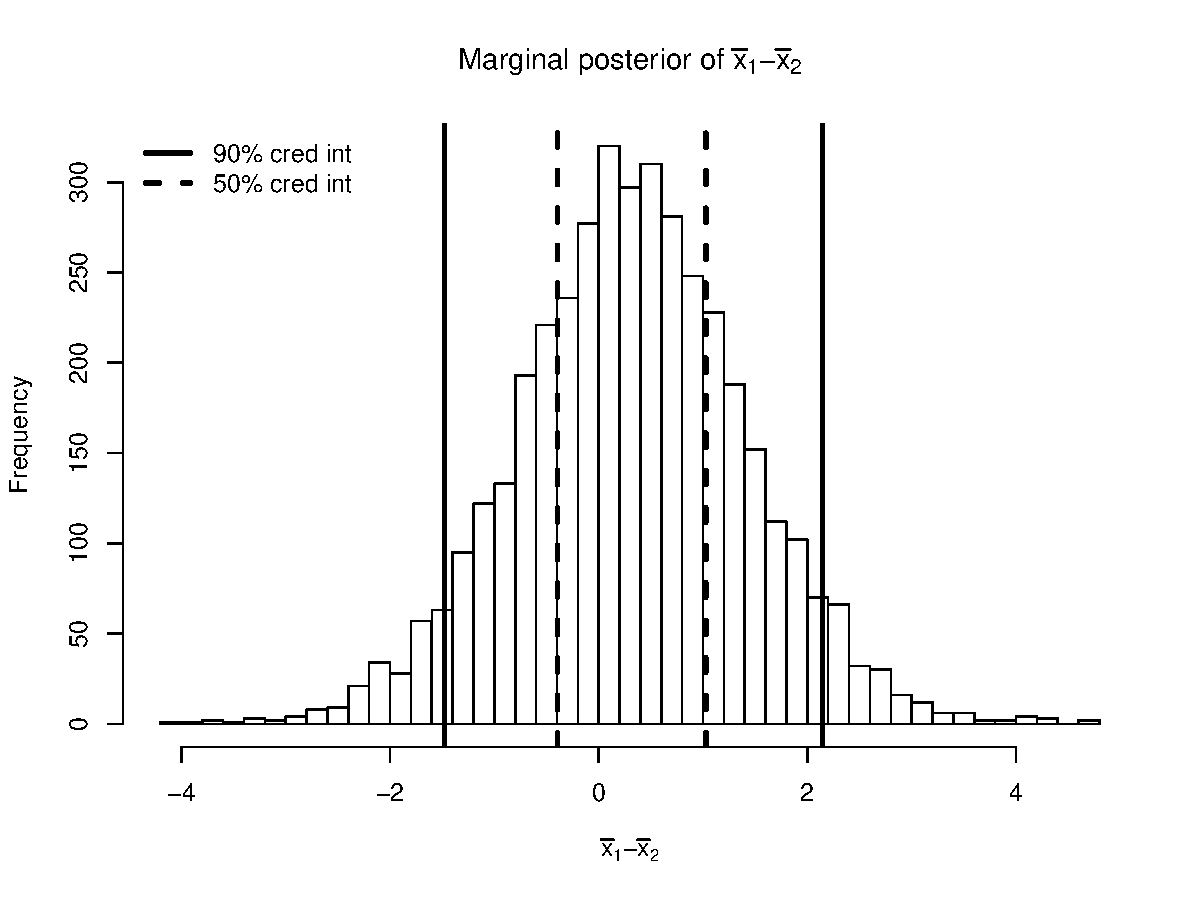
\includegraphics[trim={0cm 0cm 0cm 0cm}, clip, scale=0.4]{../figs/norm2.pdf}
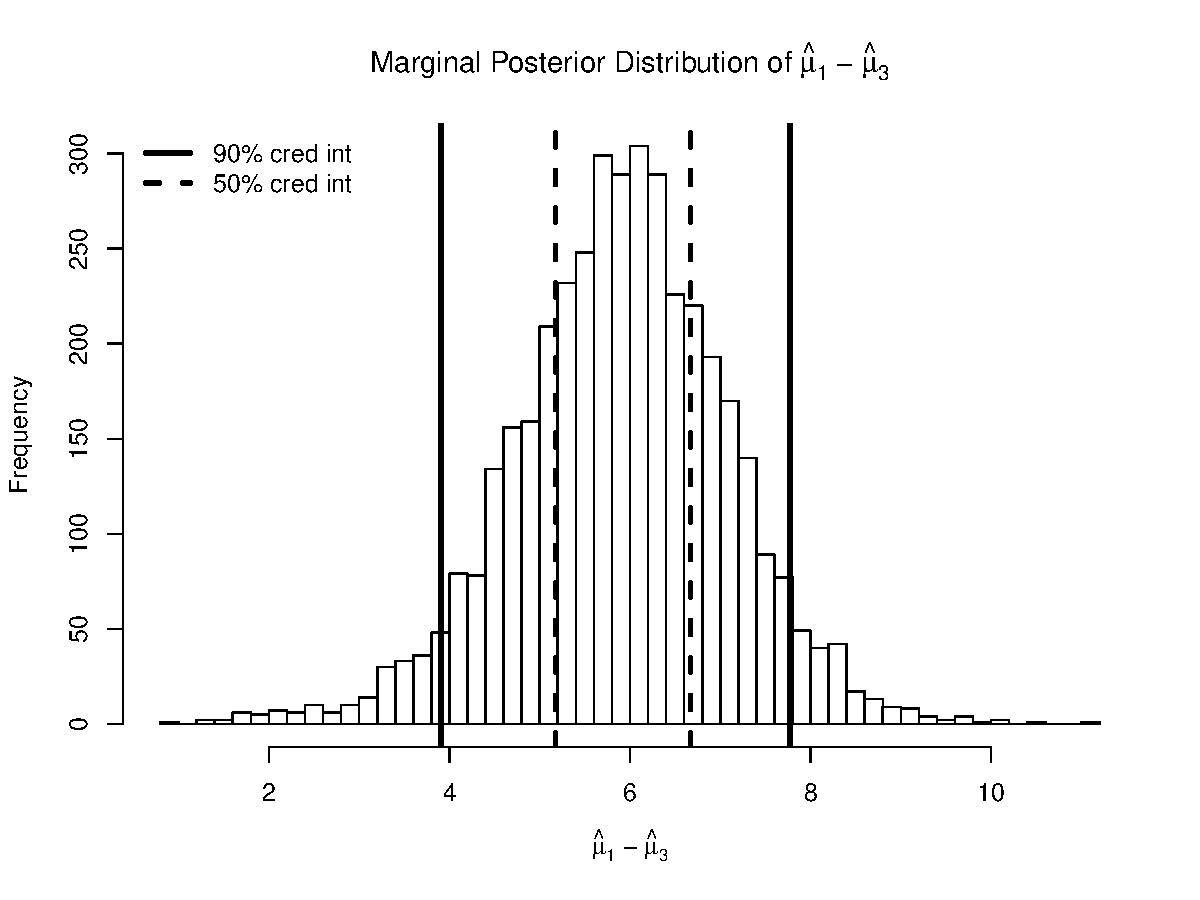
\includegraphics[trim={0cm 0cm 0cm 0cm}, clip, scale=0.4]{../figs/norm3.pdf}
\footnotesize
\end{minipage}
\end{figure}

\pagebreak

\section{Appendix A - Bayesian Alternative to Binomial test}

The example outlined above involves the t-test which requires the data to be noramally distributed. Here we look into inference on count data, specifically data generated from the binomial distribution. In Frequentist statistics the test used to compare the probability of success between some realized data sample and a hypothesized value is the \emph{binomial test}. This is commonly used in \textbf{A/B testing} where researchers are interested in the determining whether there is a substantial difference in the click through rate of an online advertising campaign. \\

\noindent In the context of the binomial test the p-value is calculated as,

\begin{align*}
d &= Bin(\hat{x}, N, p_0) \\
\mbox{p-value} &= \sum_{x=0}^{N}Bin(k, N, p_0) \mbox{ s.t. } Bin(x, N, p_0) \leq d
\end{align*}

\noindent where $x$ is the number of successes, $\hat{x}$ is the number of observed success (datum), $N$ is the number of trials, and $p_0$ is the hypothesized value for the probability of success. \\

\noindent As an example consider $x = 7$, $N = 10$, and $p_0 = 0.8$. Using the method described above we get a p-value of approximately 0.4296, preventing us from rejecting the null hypothesis that the probability of success is different from 0.8. This result is illustrated in the figure below which shows the density evaluated for each success under the hypothesized success rate. The densities that constitute the p-value are in red.

\begin{figure}[H]\caption[]{Empirical Distribution of t-Statistic}
\centering
\begin{minipage}{0.6\linewidth}
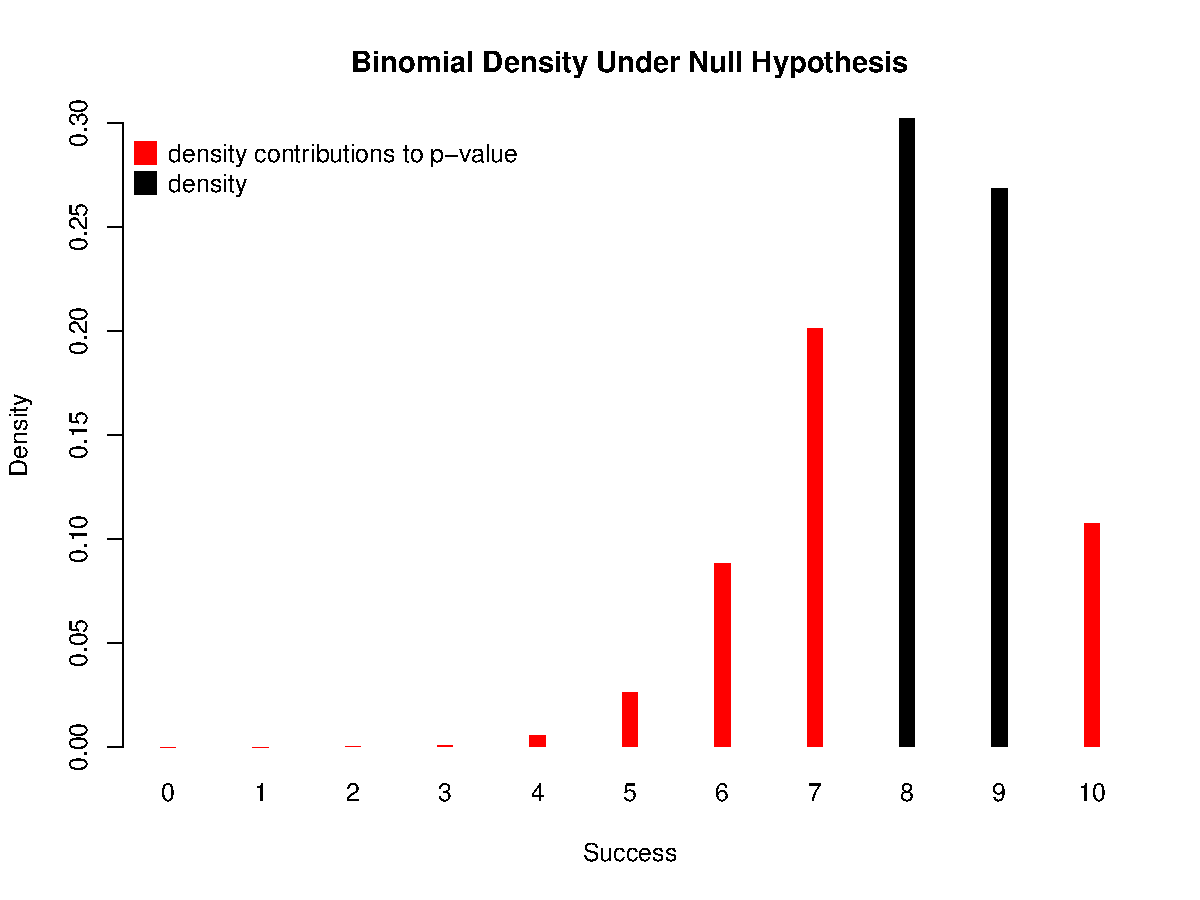
\includegraphics[trim={0cm 0cm 0cm 1.5cm}, clip, scale=0.6]{../figs/bintest_dist.pdf}
\end{minipage}
\end{figure}

\noindent As mentioned in this paper, the Bayesian approach involves modeling the data with prior information. In this case, the model is $7 \sim Bin(10, p)$ with a prior distribution defined on $p$ (the Beta distribution is typically used). We can then compute the quantiles and determine whether the estimated probability of success $p$ is different from the hypothesized value $p_0 = 0.8$. In this case we cannot conclude that the estimated probability of success is different from 0.8 since 90\% the time the parameter is between 0.44 and 0.86, conditional on the data and prior information. This result is illustrated below. \\

\begin{figure}[H]\caption[]{Posterior distribution of $p$}
\centering
\begin{minipage}{0.6\linewidth}
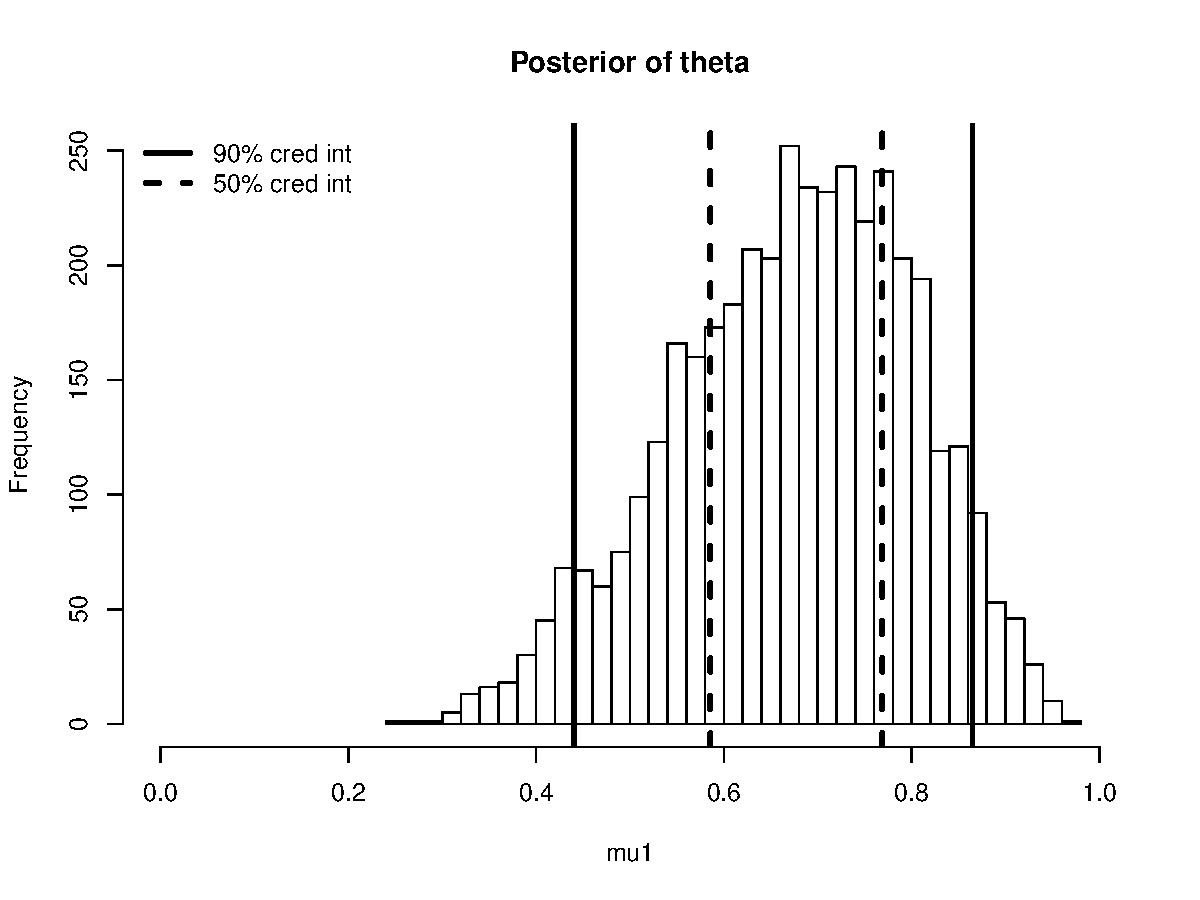
\includegraphics[trim={0cm 0cm 0cm 1.5cm}, clip, scale=0.6]{../figs/bin1.pdf}
\end{minipage}
\end{figure}

\noindent Note that the hypothesized value 0.8 is not in the 50\% credible interval (0.56, 0.78). This means that 50\% of the time the success rate parameter will be different from 0.8. It is up to the researcher to determine which interval is appropriate given the problem at hand. Under the context of the click through rate example, this would mean that there is a 50\% chance we will not observe a click through rate of 0.8.\\

\noindent This approach can easily be extended to multiple observations. The only difference would be to model the vector of successes (instead of a single observation) and a vector of associated trials. The inference on the probability of success parameter associated with these data would be the same. \\

\end{document}
